\section{Two Proofs}



The Gauss-Bonnet theorem for regular surfaces states

\begin{theorem}[The Continuous Gauss-Bonnet Theorem] \label{thm:g-b-c}

If $M$ is a regular surface with boundary $\partial M$ then
	$$\int_{M} K dA+ \int_{\partial M} k_g ds + \sum_i \beta_i= 2\pi \chi(M)$$
	where  $K$ is Gaussian curvature,
	 $k_g$ is the geodesic curvature,
	 each $\beta_i$  is an exterior angle at a vertex of the boundary and
	$\chi$ is the Euler characteristic.
\end{theorem}


The  Gauss-Bonnet theorem tell us that, if we add up curvature
at each vertex the sum will be $2\pi$ times to Euler characteristic.
The curvature at each vertex is computed by considering a 'local' neighborhood
around the vertex and we learn global topological information. Thus, the Gauss-Bonnet 
theorem is an example of a local to global principle. 
Conversely, if we know the Euler characteristic we can learn about the curvature
at individual points. We will often use the theorem to prove the existence of
a vertex with a desirable amount of curvature.



\subsection{Index Theorem Proof}
We now include a proof of a combinatorial version of the theorem due to Banchoff
\cite{banchoff_critical_1970}. Our proof will use another local to global theorem,
the Poincar\'e index theorem, which we now introduce.

A \emph{tangent vector field} on a surface is an assignment of a tangent
vector to each point. A vector field is \emph{smooth} if the tangent vectors
varies continuously. See \figref{vector-field}.
Given a vector field $X$, if $X$ has isolated zeros, we
can use $X$ to compute the Euler characteristic.
As in \thmref{euler}, we place a positive charge at each vertex, a negative charge on
each edge, and a positive charge inside of each face of the triangulation, and flow
the charges using $X$. If $z$ is a zero of $X$, the \emph{index} of $X$ at $z$,
is the sum of the charges inside of the polygon containing $z$ and is denoted
$i(X,z).$

 \begin{figure}[htb]
         \centering
         \includegraphics[width=5cm]{background/vector-field}
	\caption{An example of a vector field.
	\label{fig:vector-field}}
 \end{figure}
 

\begin{theorem}[Poincar\'e Index Theorem] \label{thm:poincare-index}

If $M$ is a regular triangulated surface and $X$ a vector field on $M$ with isolated zeros,
the Euler characteristic of $M$ is 
$$\chi(M)=\sum_{z\in \text{zeros}}i(X,z).$$
\end{theorem}

\begin{proof}
We subdivide and perturb the triangulation so that all of the zeros are inside of a unique face.
It is not obvious that this is possible but we will not prove it here.
We also assume that $X$ is transverse to each edge.
If a triangle does not contain a zero, then the sum of the charges
contributed by the flow is zero.
Thus, all charges that contribute to the Euler characteristic
results from polygon's that contain a zero.
The sum of the charges in a polygon that contains a zero is the definition of the sindex
of the zero.

\end{proof}

We proceed with the proof of \thmref{g-b-c}. 

\begin{proof}
Given a surface embedded in $\R^3$ consider a line $\ell$ and define a 
linear height function $h:M \to \R$
to be the projection of all of $\R^3$ on to the line $\ell$. A point $p$ on $M$
is a \emph{critical point} for $\ell$ if the tangent plane at $p$ is perpendicular to $\ell$.
All points on $M$ that are not critical are \emph{ordinary point}.
Critical points can be classified into three categories, maxima, minima, and saddle points.
Flow in the downward direction on $\ell$ defines a vector field on $M$.
Critical points of the height function are zeros of the vector field.
Moreover, $i(p,h)=1$ if $p$ is a  local maximum or minimum and $i(p,h)=-1$ is $p$ is a saddle point.
An example is shown in \figref{torus-total}.


For an ordinary point $q$, the tangent plane at $q$ is not horizontal. 
Now consider the plane perpendicular to $\ell$ and through $q$, this plane
divides a `small' neighborhood $U$ of $q$ into two pieces and intersects
a `small' circle about $q$ in two points.
Therefore, the index at a point $p$ can be defined as follows.
Let $\mathcal{C}$ denote the number of points a plane through $p$ perpendicular
to $h$ meets a `small' circle around $p$, then 
$$i(p,h)=1-\frac{1}{2}\mathcal{C}.$$

If we are considering polyhedral surfaces, then each point inside of a face or an edge
is ordinary, since we assumed that no face or edge is perpendicular to our line $\ell.$
A vertex can be any of the three types of critical points.
So, for each vertex $v$, we cut out the triangles incident to it. This collection of triangles
is called the \emph{star}$(v)$ of $v$. 
The index is then equal to the number of triangles in star$(v)$ with vertices
straddling the plane perpendicular to our surface at $v$. For these triangle,
we call $v$ the middle vertex and we can write the index as

$$i(v,\ell)=1-\frac{1}{2} \left(\text{number of triangles with } v \text{ middle for } \ell\right).$$



For a triangulated surface, each face is a triangle and has three edges and each
edge is incident to two faces, so
\begin{equation} \label{eqn:faces-edges}
	3F=2E.
\end{equation}

Putting our pieces together, we have
\begin{align}
\sum_{v\in M}i(v,\ell) &=\sum_{v\in M} \left(1-\frac{1}{2}(\text{number of triangles with } v \text{ middle for } \ell)\right),  \\ \nonumber
       &=V - \frac{1}{2}\sum_{v\in M} \left(\text{number of triangles with } v \text{ middle for } \ell\right), \\ \nonumber
       &=V-\frac{1}{2} F \text{ ,because each triangle has exactly one middle vertex for  } \ell,\\ \nonumber
       &= V-\frac{1}{2}(2E-2F), \text{by \eqnref{faces-edges}}\\ \nonumber
       &=V-E+F. \nonumber 
\end{align}
The above equations, together with \thmref{poincare-index}, prove the Gauss-Bonnet Theorem.

\end{proof}

 \begin{figure}[htb]
         \centering
        \begin{subfigure}[b]{0.3\textwidth}
         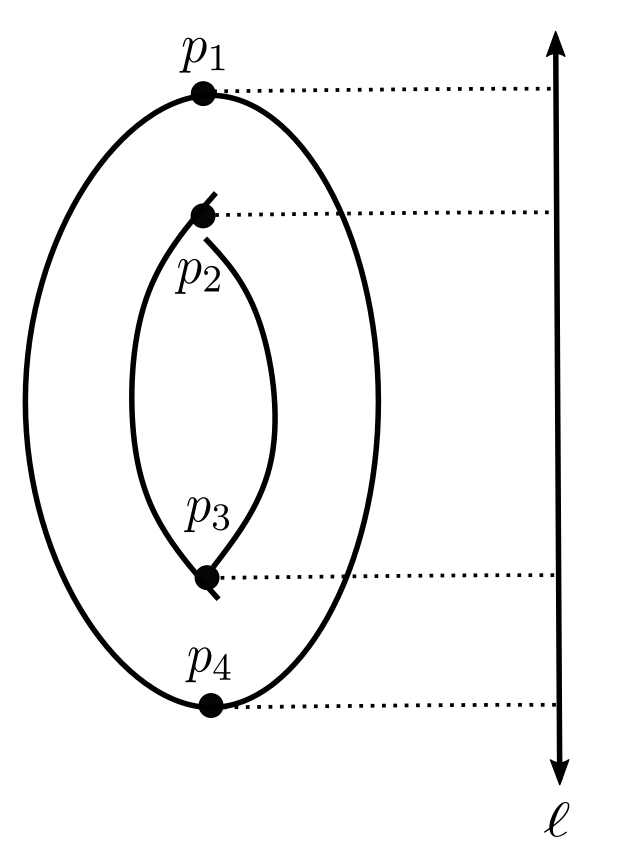
\includegraphics[width=\textwidth]{chapter-3/torus}
         \subcaption{The tours a line $\ell$ with four critical points.}
 	 \label{fig:torus-ell}
       \end{subfigure}\\
         \begin{subfigure}[b]{0.21\textwidth}
         \includegraphics[width=\textwidth]{chapter-3/torus-top}
         \subcaption{Local to $p_1$.}
          \label{fig:max}
         \end{subfigure}
          \begin{subfigure}[b]{0.21\textwidth}
         \includegraphics[width=\textwidth]{chapter-3/saddle1}
         \subcaption{Local to $p_2$.}
          \label{fig:saddle1}
         \end{subfigure}
         \begin{subfigure}[b]{0.21\textwidth}
         \includegraphics[width=\textwidth]{chapter-3/saddle2}
         \subcaption{Local to $p_3$.}
          \label{fig:saddle2}
         \end{subfigure}
         \begin{subfigure}[b]{0.21\textwidth}
         \includegraphics[width=\textwidth]{chapter-3/torus-bottom}
         \subcaption{Local to $p_4$.}\label{fig:min}
         \end{subfigure}
		\caption{(\subref{fig:torus-ell}) A tours and line $\ell$. There are four critical points.
 		(\subref{fig:max}) The critical point $p_1$ is a maximum and $i(p_1,h)=1$.
		(\subref{fig:saddle1}) The critical point $p_2$ is a saddle and $i(p_1,h)=-1$.
		(\subref{fig:saddle2}) The critical point $p_3$ is also a saddle and $i(p_1,h)=-1$.
		(\subref{fig:min}) The critical point $p_4$ is a minimum and $i(p_1,h)=1$.
 		\label{fig:torus-total}}
 \end{figure}


The above proof can be extended to smooth surface and to surfaces with boundary.
Next, we give a significantly different proof the Gauss-Bonnet theorem. 


%%%%%Dump below

\subsection{Triangle Cancelation Proof}
\label{sec:proof}


We present a proof of the Gauss-Bonnet theorem similar to the proof given by Upadhyay \cite{upadhyay2015}.
First, we consider the case where our surface does not have a boundary.
We then extend this case to surfaces with boundary.
\begin{theorem}[Discrete surfaces without boundary]\label{thm:g-b-discete-bdy}
For a triangulated surface $S$ without boundary
$$\sum_{v\in V} K(v)=2\pi \chi(S)$$
where $K(v)$ is the discrete curvature.
\end{theorem}

\begin{proof}

For each vertex $v$ in $S$,
let $deg(v)$ denote the number of edges incident to $v$, let $\alpha_1,\alpha_2,\ldots,\alpha_{\deg{(v)}}$ denote the angles
containing $v$ and let $\xi_i=\pi-\alpha_i$ for each $i$.
By \eqnref{discrete-curvature-complement-angle}, 
the discrete Gaussian curvature at a $v$ is
 $$K(v)=(2-\deg{(v)})\pi +\sum_{i=1}^{\deg{(v)}} \xi_i.$$
Summing over all vertices in $S$ gives
$$\sum_{v\in V} K(v)=\sum_{v\in V}2\pi - \sum_{v\in V}\deg{(v)}\pi+\sum_{v\in V}\sum_{i=1}^{\deg{(v)}} \xi_i.$$
The first term on the right hand side is $2\pi |V|$. Each edge is incident with two vertices, so the second term is $2\pi |E|$. 
In the third term, we rewrite $\xi_i$ as $\pi-\alpha_i$.

$$ \sum_{v\in V}\sum_{i=1}^{\deg{(v)}} \beta_i= \sum_{v\in V}\sum_{i=1}^{\deg{(v)}} (\pi-\alpha_i).$$
We can reorganize this sum as follows, instead of summing the angles around each vertex we can sum the angles in each face.
Each angle in $S$ is still being counted exactly once. 
Since each face is a triangle, this gives
$$\sum_{v\in V}\sum_{i=1}^{\deg{(v)}} (\pi-\alpha_i)=\sum_{f\in F}\sum_{i=1}^3(\pi-\alpha_i).$$
Since each face is a triangle the sum of the three angles is $\pi$,
so $\sum_{i=1}^3(\pi-\alpha_i)=3\pi-\pi=2\pi.$
Thus, $$\sum_{v\in V} K(v)=2\pi |V|-2\pi |E|+2\pi |F|=2\pi \chi(S)$$ as desired.
\end{proof}

Next, we extend the above proof to the case where $S$ has a boundary
by gluing a copy of $S$ to itself along the boundary.

\begin{theorem}[Discrete surfaces without boundary]\label{thm:g-b-discete}
For a combinatorial surface $S$ with boundary

$$\sum_{v\in S_{\text{int}}} K(v)+\sum_{v\in\partial S}k_g(v)=2\pi \chi(S)$$
where $K(v)$ is the discrete curvature and $k_g(v)$ is the discrete geodesic curvature.
\end{theorem}

\begin{proof}
Take a copy of $S$ and attach it to itself along the boundary.
This creates the surface $2S$ without boundary. Notice,
when we copy $S$ we create two copies of the boundary, and when
we glue we remove one copy of the boundary.
Thus, $$\chi(2S)=2\chi(S)-\chi(\partial S).$$
Since, $\partial S$ is piecewise linear the number of vertices and
edges are equal and there are no faces, so $\chi(\partial S)=0$
and 

\begin{equation} \label{eqn:glue}
\chi(2S)=2\chi(S).
\end{equation}
For $v$ a vertex on the boundary, $k_g(v)$ is half
the discrete Gaussian curvature of $v$ in $2S.$
Thus,

$$\sum_{v\in 2S}K(v)=2\left(\sum_{v\in S_{\text{int}}}K(v)+\sum_{v\in \partial S} k_g(v)\right) =2\pi  \chi(2S).$$
Applying \eqnref{glue},

$$\sum_{v\in S}K(v)+\sum_{v\in \partial S} k_g(v)=2\pi  \chi(S)$$
as desired.

\end{proof}



